\documentclass{beamer}
\usepackage{graphicx}
\usepackage{caption}
%\usepackage{subcaption}
\usepackage{color}
\usepackage{amssymb}
\usepackage{xcolor}
\usepackage{wrapfig}
\usepackage{amsmath}
\usepackage[
backend=bibtex,
sorting=none,
style=authoryear
]{biblatex}
\addbibresource{bibliography.bib}

\defbibenvironment{nolabelbib}
  {\list
     {}
     {\setlength{\leftmargin}{\bibhang}%
      \setlength{\itemindent}{-\leftmargin}%
      \setlength{\itemsep}{\bibitemsep}%
      \setlength{\parsep}{\bibparsep}}}
  {\endlist}
  {\item}

\setbeamertemplate{navigation symbols}{}
\usetheme{CambridgeUS}
\usecolortheme{beaver} 

\beamersetuncovermixins{\opaqueness<1>{25}}{\opaqueness<2->{15}}

%\pgfdeclareimage[height=2cm]{i4}{pic/acat.pdf}


%\author[Dzmitry Makatun]{\textbf{Dzmitry~Makatun} \inst{1} $^{,}$ \inst{2}}

\author[Dzmitry Makatun]{\textbf{Dzmitry~Makatun} \inst{1} \inst{3} \and J\'er\^ome~Lauret\inst{2}\\ \and Michal~\v{S}umbera \inst{1} \and Hana~Rudov\'a \inst{4}}
\title[Distributed data production planning]{Model for planning of distributed data production} 
\institute [KM, FJFI]
{ 
  \inst{1}%
  Nuclear Physics Institute, Academy of Sciences, Czech Republic
  \pgfdeclareimage[height=2cm]{i1}{pic/ujf.pdf}   
  \and
  \inst{2}%
  Brookhaven National Laboratory, USA
  \pgfdeclareimage[height=2cm]{i2}{pic/STAR.pdf}
  \and
  \inst{3}
Czech Technical University in Prague, Czech Republic  
\pgfdeclareimage[height=2cm]{i3}{pic/ctu.pdf} 
\and
\inst{4}
Faculty of Informatics, Masaryk University, Czech Republic
\pgfdeclareimage[height=2cm]{i6}{pic/fjfi.pdf}
\pgfdeclareimage[height=2cm]{i8}{pic/doe.pdf}
 
\vspace{-4mm}   
  \pgfuseimage{i1}
  \pgfuseimage{i2}
  \pgfuseimage{i3}
  %\pgfuseimage{i4}
  %\pgfuseimage{i5}
  %\pgfuseimage{i6}
  %\pgfuseimage{i8}

  \vspace{-7mm}
\begin{center}
d.i.makatun@gmail.com
\end{center}
\vspace{-5mm}
  }
\begin{document}
\date{27.08.2015} 

\begin{frame}[noframenumbering]
\titlepage
\end{frame}

\begin{frame}[noframenumbering]\frametitle{Outline}
\tableofcontents
\end{frame}

\section{Introduction}
\subsection{Data processing in High Energy Physics (HEP)}

\begin{frame}\frametitle{Computations in HEP: what do we compute?}
\begin{figure}
\begin{center}
%\vspace{-1 cm}
\includegraphics[ height=0.4\textheight]{pic/rhic.jpg}
\hspace{0.5cm}
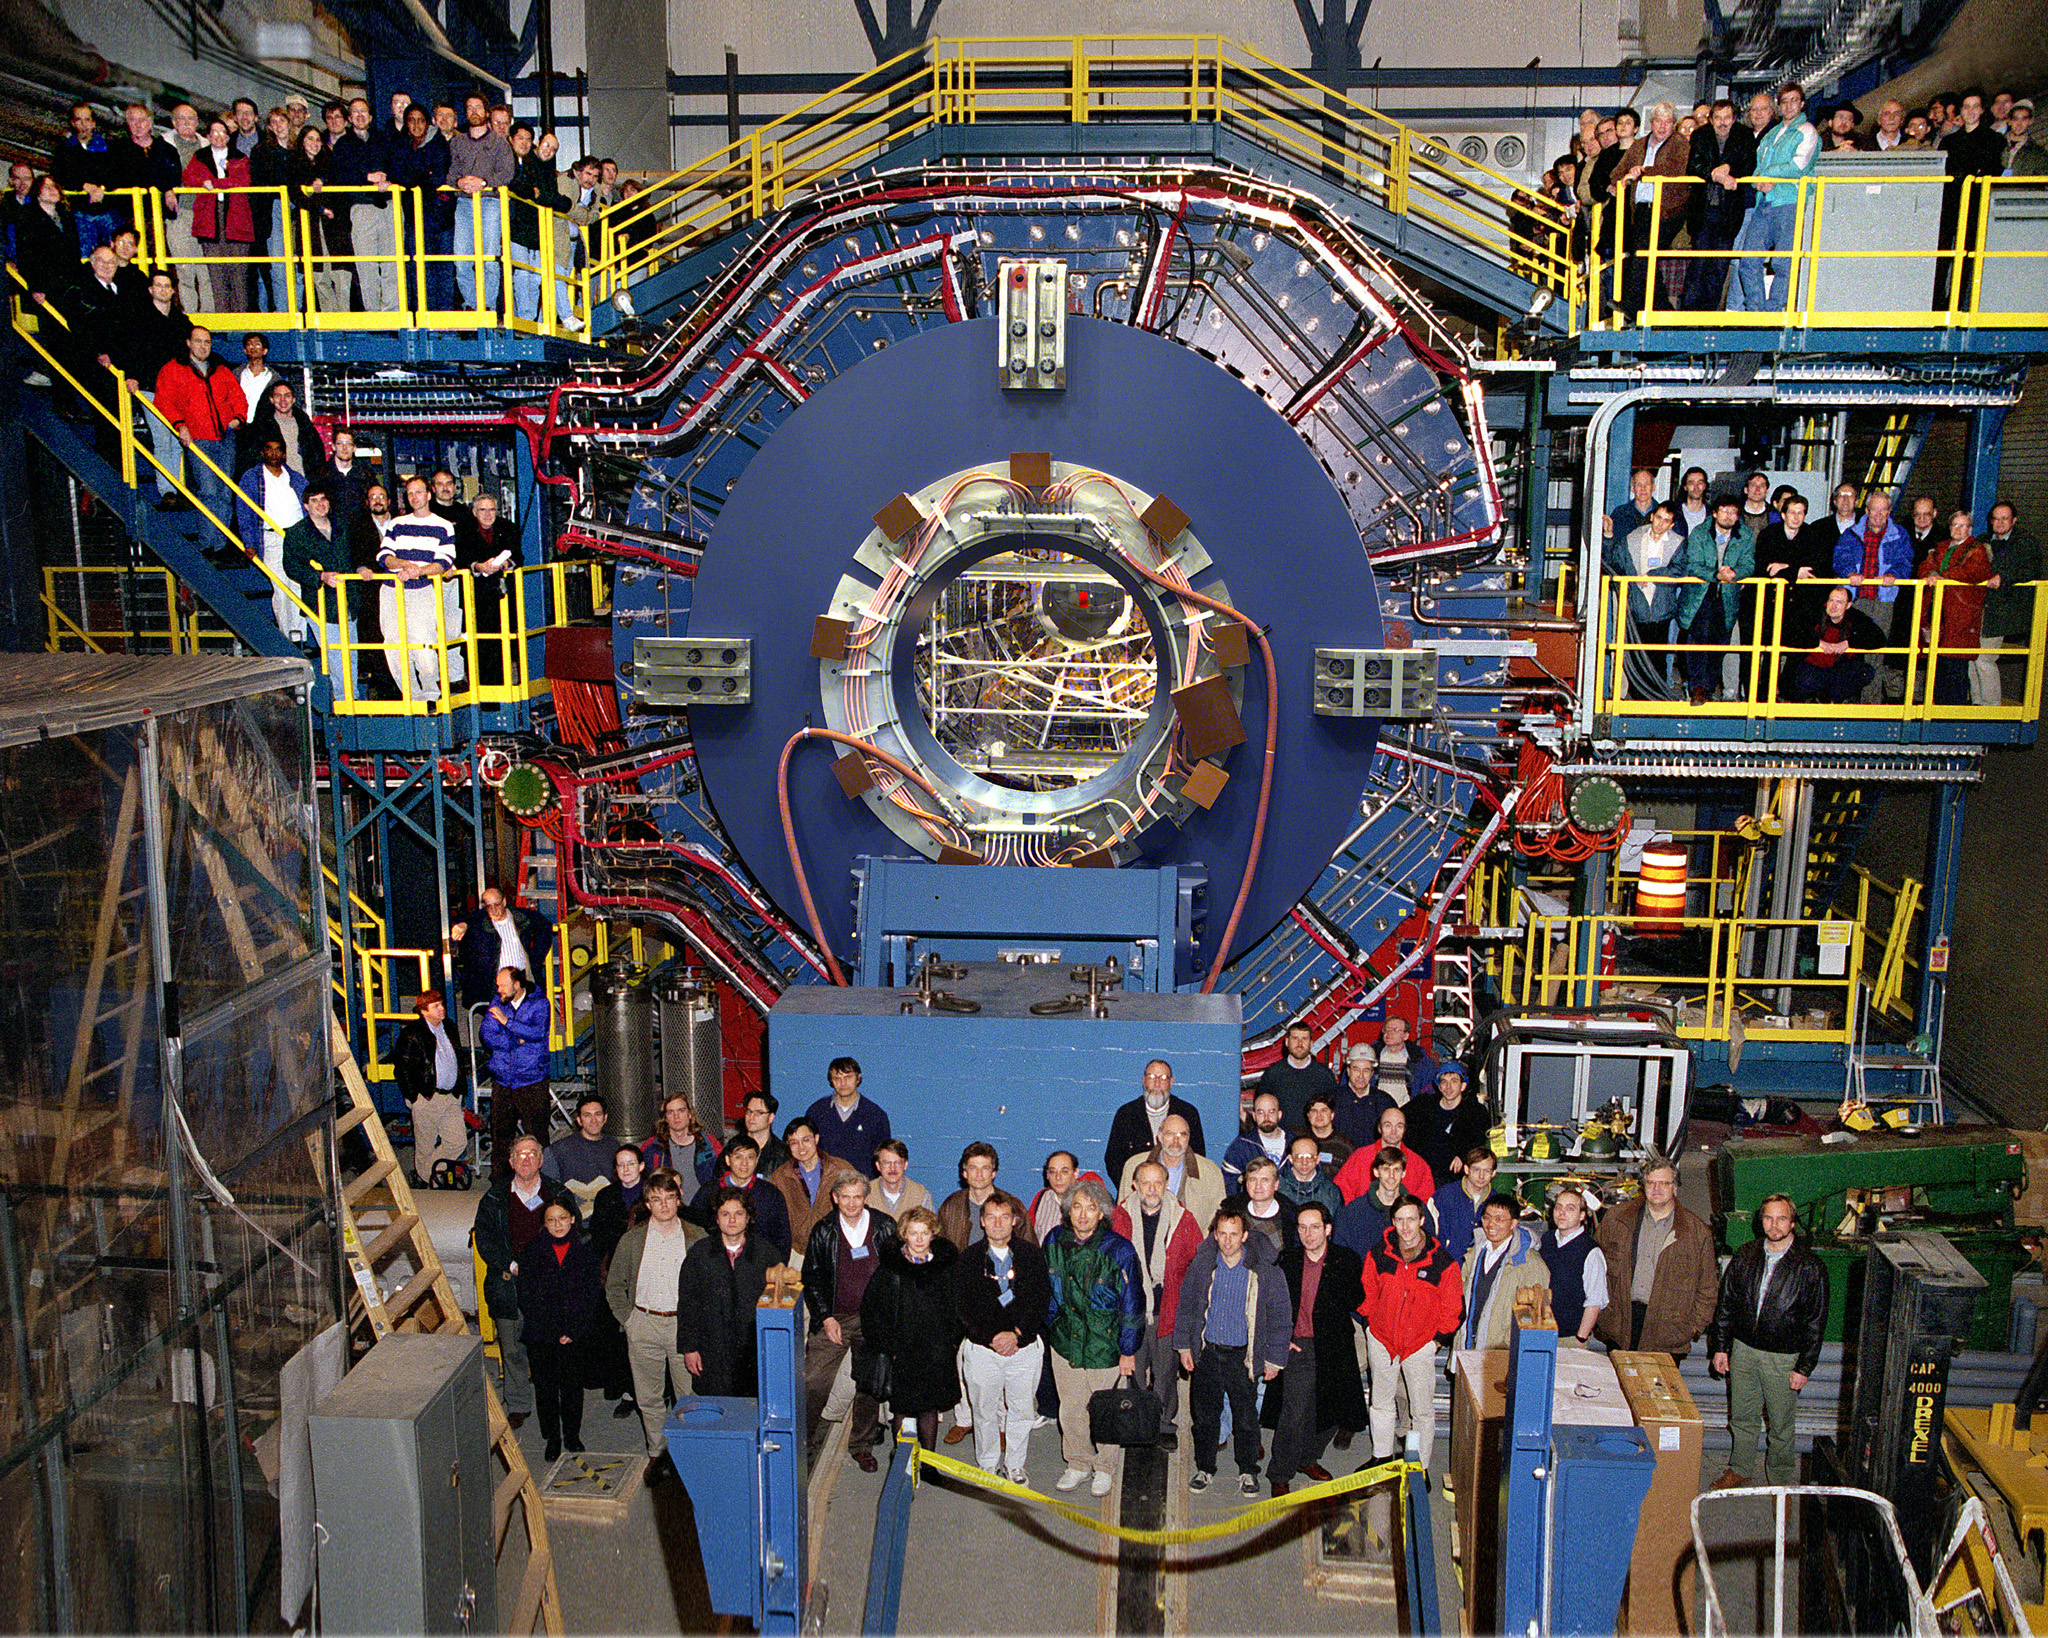
\includegraphics[ height=0.4\textheight]{pic/star.jpg}
\end{center}
\end{figure}
\vspace{-1 cm}
\begin{block}{}
		\begin{itemize}
			\item Brookhaven National Laboratory (\textbf{BNL}) Long Island, NY, USA
			\item Relativistic Heavy Ion Collider (\textbf{RHIC}). In Gold-Gold ion collisions a quark-gluon plasma is created to study the primordial form of matter that existed in the universe shortly after the Big Bang.
			\item Solenoid Tracker at RHIC (\textbf{STAR}). Collisions occur millions of times per second. Events of size 200 MB are processed at input rates up to 100Hz. Output data rate is $\sim$ \textcolor{red} {30 MB/sec}.
		\end{itemize}
 	\end{block}
\end{frame}

\begin{frame}\frametitle{Computations in HEP: how do we compute?}
\begin{block}{}
\textbf{Data Production:} The raw output data is processed to reconstruct events ($\sim$ ones).\\
\textbf{User Analysis:} Then the reconstructed events are analyzed by scientists to discover new physics (each file many times).\\
All the data: raw, reconstructed and analysis output are stored.\\
31 PB of data stored on tape, $\sim$ 12 000 jobs running simultaneously (at RCF only).\\

 	\end{block}
\begin{figure}
\begin{center}
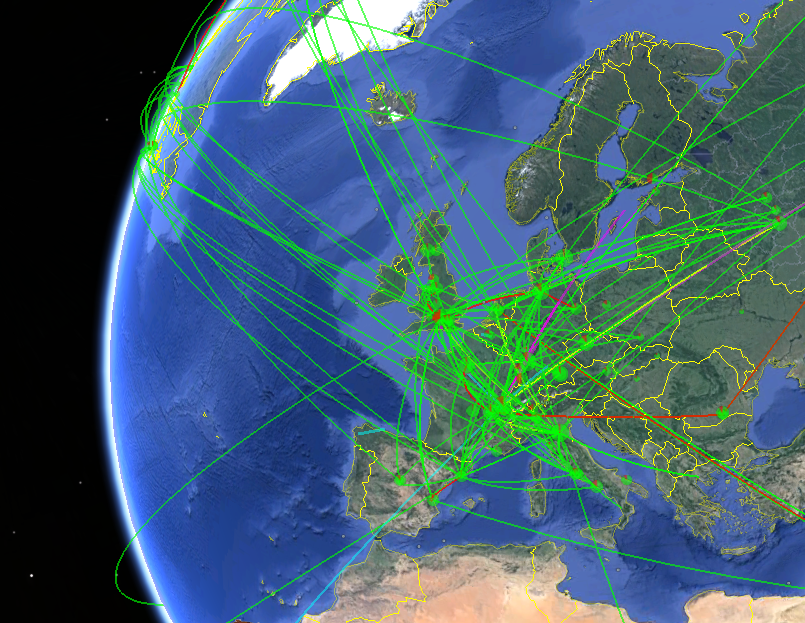
\includegraphics[ height=0.35\textheight]{pic/grid-net.png}
\hspace{0.1cm}
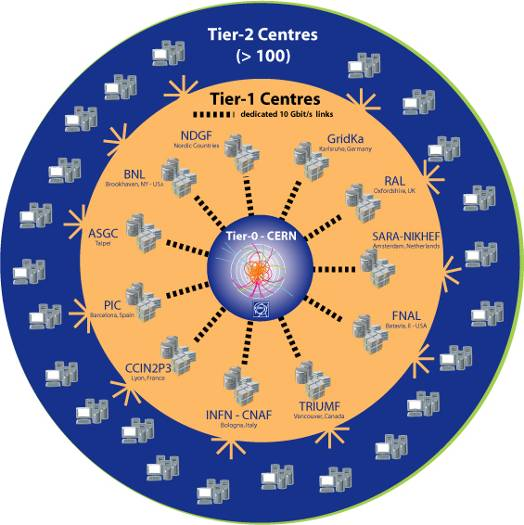
\includegraphics[ height=0.35\textheight]{pic/tiers.jpg}
\hspace{0.1cm}
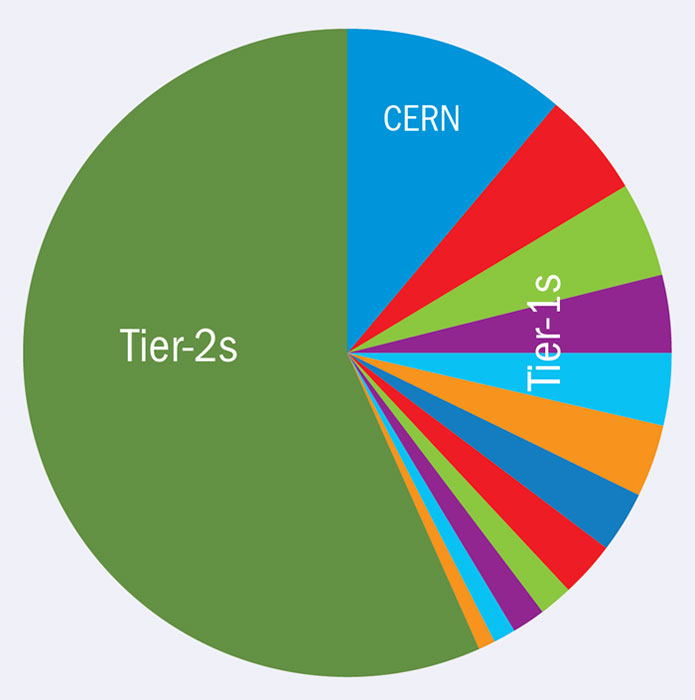
\includegraphics[ height=0.35\textheight]{pic/cern-tier-chart.jpg}
\end{center}
\end{figure} 	
\end{frame}


\begin{frame}\frametitle{Case 1: Data production. Planning remote site usage }
 	\begin{columns}[c] % the "c" option specifies center vertical alignment
    \column{.6\textwidth} % column designated by a command 	
    \begin{footnotesize}
    \vspace{-11mm}
	\begin{block}{}
		\begin{itemize}
		\item RAW data is located at BNL.
		\item Computational resources are available at BNL and several remote sites.
		\item 1 job per file.
		\item 1 CPU per job. 
		\item Input size $\approx$ Output size.
		\item Output file has to be transferred back to BNL.
		\item \textbf{How should we distribute a given set of files between sites to complete the processing faster?}
		\end{itemize}
 	\end{block} 	
 	
 	\begin{block}{}
 	Manually adjust the number of remote jobs to meet the network throughput, \textbf{but} what if:
		\begin{itemize}
		\item[-] More sites
		\item[-] Changing network load
		\end{itemize}
	This should be automated.
 	\end{block}  	     

 	\end{footnotesize}
 	\column{.4\textwidth}
 		\vspace{-5mm}
		\begin{figure}   
				\includegraphics[trim = 25mm 10mm 0mm 30mm, clip, width=1.2\textwidth]{pic/Data_production_schema2.pdf}
		\end{figure} 	 	
 	\end{columns}
\end{frame}

\begin{frame}\frametitle{Case 2: Data production. Optimization }
 	\begin{columns}[c] % the "c" option specifies center vertical alignment
    \column{.5\textwidth} % column designated by a command 	
    \begin{footnotesize}
    \vspace{-20mm}
	\begin{block}{New dimensions of the problem}	
		\begin{itemize}		
			\item Several possible data sources.
			\item Real network topology: shared links, \textbf{links between remote sites}.
			\item Limited storage at sites.
			\item \textbf{Which file source to select?}
			\item \textbf{What is the optimal transfer path?}

		\end{itemize}
 	\end{block}
		\begin{block}{Example: data-production at ANL  \textcolor{black}{[\cite{Balewski}]}}	
		\begin{itemize}
			\item ANL: many CPU's, but slow connection and small disk space.
			\item NERSC: fast connection, large disk.
			\item Optimization: Feed ANL from both BNL and NERCS sites.		

		\end{itemize}
 	\end{block}
 	\end{footnotesize} 
 	\column{.45\textwidth}
		\begin{figure}
			\begin{center}
			    \vspace{-15mm}
				\includegraphics [width=1.2\textwidth]{pic/Data_production_schema_ANL2.pdf}
			\end{center}
			\end{figure} 	 	
 	\end{columns}
\end{frame}


\begin{frame}\frametitle{Case 3: User analysis }
 	\begin{columns}[c] % the "c" option specifies center vertical alignment
    \column{.5\textwidth} % column designated by a command
 	\begin{small}
 	\vspace{-10mm}
	\begin{block}{New dimensions of the problem}
		\begin{itemize}
			\item Many copies of files exist.	
			\item Each file can be requested by multiple jobs.
			\item The size of output of analysis is negligible compared to input size.
			\item The processing time estimates  are imprecise.
			\item \textbf{When and where to replicate the data?}
		\end{itemize}
 	\end{block} 	
 	\end{small}
 	\column{.45\textwidth}

		\begin{figure}
			\begin{center}
			    \vspace{-15mm}
				\includegraphics[ width=1.15\textwidth]{pic/user_analysis.pdf}
			\end{center}
			\end{figure} 	 	
 
 	\end{columns}
\end{frame}

\subsection{Load balancing}
\begin{frame}\frametitle{Existing solutions (load balancing in HENP)} 	
\begin{block}{Batch System + Distributed Data Management System (Independent)}  
		\begin{itemize}
			\item PBS, Condor. [Pull a job from the global queue]
			\item Xrootd, DPM. [The site which replies the first is selected as a source] 			
		\end{itemize}
 	\end{block} 	
\begin{block}{Data Trains (For user analysis)}	
	 \begin{itemize}
	 \item Group jobs by input data $\longrightarrow$ preplace data $\longrightarrow$ start jobs simultaneously $\longrightarrow$ kill latest x\% of jobs. 
	 \item Train runs periodically ($\sim$ ones per day).  
 	 \item Controlled by train operators. 
 	  \end{itemize}
\end{block}
\begin{block}{Globus (Decoupling jobs and transfers)} 	
\begin{itemize}
 	 \item Sends jobs to data.  
 	 \item Replicate most "popular" files. Relies on usage history.
 	 \item Where to replicate? When to replicate? No transfer planning.
 	 \end{itemize}
\end{block} 	 
\end{frame}


\section{Data production planning}
\begin{frame}\frametitle{Data production problem}
	\begin{block}{Data production:}
		\begin{itemize}
			\item Each input file is processed ones.
			\item One CPU per job.
		\end{itemize}
 	\end{block}  

 		\begin{block}{Task}
Create a global scheduler for Grid which will reason about:\\
\hspace{1cm} 1.data~transferring, \hspace{1cm} 2.~CPU~allocation,\hspace{1cm} 3.~data~storage.  
\end{block}
\begin{block}{Optimization}  
		\begin{itemize}
			\item None of the resources (network links, data storages and CPUs) are over-saturated at any moment of time.
			\item The jobs are executed  where the data is pre-placed.
			\item Output data is transferred back to the central storage.
			\item No excessive transfers or data replication.
		\end{itemize}
 	\end{block}
	
\end{frame}


\subsection{Network flow model}
\begin{frame}\frametitle{Network flow model} 
  \begin{block}{Idea}
    Plan resource load only and then distribute particular jobs accordingly.
  \end{block}

  \begin{block}{Network flow model}
    \begin{itemize}
      \item $\Delta T$ - planning time interval
      \item $Flow$ - amount of data to be transferred
      \item link capacity - $bandwidth \cdot \Delta T$.
    \end{itemize}
  \end{block}    
  Knowing data distribution at the beginning of $\Delta T$,\\
  \textbf{how much data should be transferred over each network link?}
  
    \begin{block}{Sub-problems:}
    \begin{itemize}
      \item Input
      \item Otput
    \end{itemize}
  \end{block}  
  
  Network flow maximization problem can be solved within polynomial time.
\end{frame}

\begin{frame}\frametitle{Input transfer planning: How much data can be transferred during the next planning interval $\Delta T$?}
Dummy edges - constraints on  storage and CPUs at each site.
\begin{figure}[h]
	\begin{center}
		\includegraphics [trim= 30mm 30mm 30mm 30mm , clip, angle =-90, width=0.7\textwidth]{pic/real_network.pdf}
	\end{center}
	\label{real_network}
\end{figure} 
\vspace{-3mm}
Output flow problem can be formulated similarly.
\end{frame}

\begin{frame}\frametitle{Solving procedure}
\begin{block}{}
Problems for input and output transfers can be solved independently under assumptions: 
\begin{itemize}
\item Full-duplex links,
\item In a steady state at each node $Processed\_input\_data= \beta \cdot Created\_output\_data$, where~$\beta = const\leq 1$.
\end{itemize}
\end{block} 

\begin{block}{Solving procedure}
\begin{enumerate}
\item Calculate capacities of (dummy) edges using monitoring data.
\item Solve the problem for output data flows.
\item Recalculate remaining network capacity.
\item Solve the problem for input transfers.
\end{enumerate}
\end{block}    
\end{frame}


\subsection{Plan execution}
\begin{frame}\frametitle{Plan execution}

\begin{columns}[c] % the "c" option specifies center vertical alignment
    \column{.6\textwidth} % column designated by a command 	

\begin{block}{}
\begin{itemize}
\item A local handler at each node receives the plan:

\begin{itemize}
\footnotesize
\item Flows of outgoing edges - how much data of each type should be send over that link.
\item Flow of dummy edges - how much data should be processed at this node.
 \end{itemize}

\item When a new file arrives, the handler decides according to the plan and current state:

\begin{itemize}
\footnotesize
 \item To process the file (to transfer over the dummy edge)
 \item OR to forward it over one of the links.  
 \end{itemize}
 \item Decrease remaining flow of the link by the size of the file after transfer.
\end{itemize}
\end{block}    


\column{.4\textwidth}
\begin{figure}[h]
		\includegraphics [trim= 30mm 30mm 30mm 30mm , clip, angle =-90, width=\textwidth]{pic/handler_process.pdf}
	\label{real_network}
\end{figure} 

\begin{figure}[h]
		\includegraphics [trim= 30mm 30mm 30mm 30mm , clip, angle =-90, width=\textwidth]{pic/handler_forwarddia.pdf}
	\label{real_network}
\end{figure} 
\end{columns}

\end{frame}



\section{Conclusion}

\begin{frame}\frametitle{Conclusion}
     Automated and scalable \textbf{planning and optimization of distributed computations} are highly required in     data intensive computational fields such as High Energy and Nuclear Physics. Resent works has revealed the potential of \textbf{global planning} for this task.
  \begin{block}{Goals of the proposed model}

    \begin{itemize}
      \item CPUs are allocated only after the input data is transferred.
      \item Feasible data distribution such that CPUs are busy with jobs while not exceeding network and storage capacities.
      \item Scalability and adaptability to changing environment.
    \end{itemize}
  \end{block}

  \begin{block}{Further plans}
    \begin{itemize}
      \item Evaluation using real log data: STAR data production, other HENP experiments, scalability tests. 
      \item Integration into distributed RMS. Deployment to the data production system of the STAR experiment. Testing, statistics collection. 
    \end{itemize}
   \end{block}
  \end{frame}


\begin{frame}<beamer>[noframenumbering]\frametitle{The end of the presentation}
\begin{center}
Thank You for Your attention.
\end{center}
\end{frame}

\section*{Bibliography}


\begin{frame}<beamer>[noframenumbering]\frametitle{References}
\nocite{Rudova}
\renewcommand*{\bibfont}{\tiny}
\printbibliography[notkeyword=my]
\end{frame}

\section*{Backup}

\end{document}
